\documentclass[11pt]{article}

\usepackage[utf8]{inputenc}
\usepackage{url}
\usepackage[margin=0.8in]{geometry}
\usepackage{graphicx}
\graphicspath{ {./images/} }
\usepackage{tabularx}
\usepackage{threeparttable}
\usepackage{pdflscape}
\usepackage{verbatim}


\title{GWAS-SSF: A GWAS Summary Statistics Format (v0.1)}
\date{19th Jul 2022}

\begin{document}
\maketitle

\newpage
\tableofcontents

\newpage

\section{Introduction}
The GWAS Catalog hosted a workshop and series of meetings between June 2020 and September 2021 with summary statistics stakeholders, including data generators, data users, data managers and bioinformaticians, representing diverse user groups. These meetings gathered requirements and identified challenges. The aim of this process was to set minimum information elements for data sharing to maximise downstream utility.

\section{Requirements}

The key requirements obtained from the stakeholders’ use cases were as follows:

\begin{enumerate}
\item Consistent representation of data to enable interoperability
\item Easily accessible metadata for summary statistics to facilitate data interpretation and re-usability
\item Unambiguously reported genetic variants for standard annotation
\item A set of mandatory (i.e.\ must be present and filled with non-null values) fields, providing the information necessary to enable a wide range of data analyses including MR and PGS development
\item A set of encouraged fields with standard headers, which are strongly recommended but not mandatory 
\item A balance between these mandatory and encouraged fields that includes essential data but does not set the bar impossibly high for the community using and implementing the standard
\item A low bioinformatics requirement for data consumers and data producers, reflecting the composition of the user community, to maximise stakeholder uptake 
\end{enumerate}

These requirements were used to define the backbone of a format---the GWAS-SSF---which will be implemented within the GWAS Catalog and promoted more widely in the community. The format has been designed to be interoperable with other major formats and resources. We continue to take public feedback on the proposed format via our github repository \url{https://github.com/EBISPOT/gwas-summary-statistics-standard} or via email to gwas-info@ebi.ac.uk.

\section{Specification}
The GWAS summary statistics format (GWAS-SSF) is composed of two files, the summary statistics data file and accompanying metadata file.

\subsection{Summary statistics data format}
The GWAS-SSF data file is a TSV flat file of tab-delimited values that can be compressed (see Figure~\ref{fig:schematic} for a schematic representation), reporting data from a single genome-wide analysis. The first line of the file contains the headers to the table. The rows after the header store the variant association data. Where permitted, values can be omitted by the presence of \texttt{NA}. There are no limits to the number of rows or columns that the table can have, however, a set of mandatory fields (defined in Table~\ref{tab:sum_stats_def}) must be present in a defined order. A file may contain additional columns beyond the set of mandatory fields. Table 1 shows some non-mandatory (encouraged) fields that may be present.


% EXAMPLE SUMSTATS
\begin{landscape}
\subsubsection{Example file data}
\scriptsize
\begin{verbatim}
chromosome  base_pair_location  effect_allele  other_allele  beta        standard_error  effect_allele_frequency  p_value  variant_id         rsid
1           869388              A              G             -0.016619   0.00806496      0.997221                 0.1      1_869388_A_G       NA
1           205811055           C              T             -0.0089589  0.00331941      0.983589                 9.7E-03  1_205811055_C_T    rs74143854
2           70478797            T              TG            0.0187528   0.00167685      0.934121                 3.5E-30  2_70478797_T_TG    rs142640435
2           27875036            TAAA           T             -0.0184003  0.00101051      0.78451                  5.7E-76  2_27875036_TAAA_T  rs774624803
23          24145170            A              G             0.00387762  0.08757958      0.627178                 2.3E-08  23_24145170_A_G    rs5949232
\end{verbatim}

\normalsize
        In this example, the summary statistics data file (TSV) has been pretty-printed to display the columns more clearly. The first line contains the column labels and every line thereafter are for variant-trait association data. Column labels and column order are in adherence to the definitions in Table 1. \textit{variant\_id} and \textit{rsid} are optional (encouraged) they are simply placed anywhere after the mandatory 8 columns. Here the effect statistic is beta, so the column label of the effect size column is \textit{beta}. The first data row represents a variant-trait association for a single-nucleotide polymorphism where the effect allele is an 'A' at the genomic location (genome assembly is given in the accompanying metadata file, see \ref{metadata_example}). No rsID was provided for this first variant, so \textit{NA} was given as the value in the \textit{rsid} column because there must be a value in all columns. The second data row shows an example where the p-value is given in scientific notation and rsID is provided. The third and fourth data rows are examples of deletions and insertions, respectively. The fifth example shows a variant located on the X-chromosome, which is mapped to \textit{23} (Table~\ref{tab:sum_stats_def}).
\end{landscape}
% ----------


% FIGURE 1
\begin{figure}[h]
 \centering
 \caption{Schematic representation of the summary statistics table. Examples of data content within each specific field are provided in Table~\ref{tab:sum_stats_def}.}
 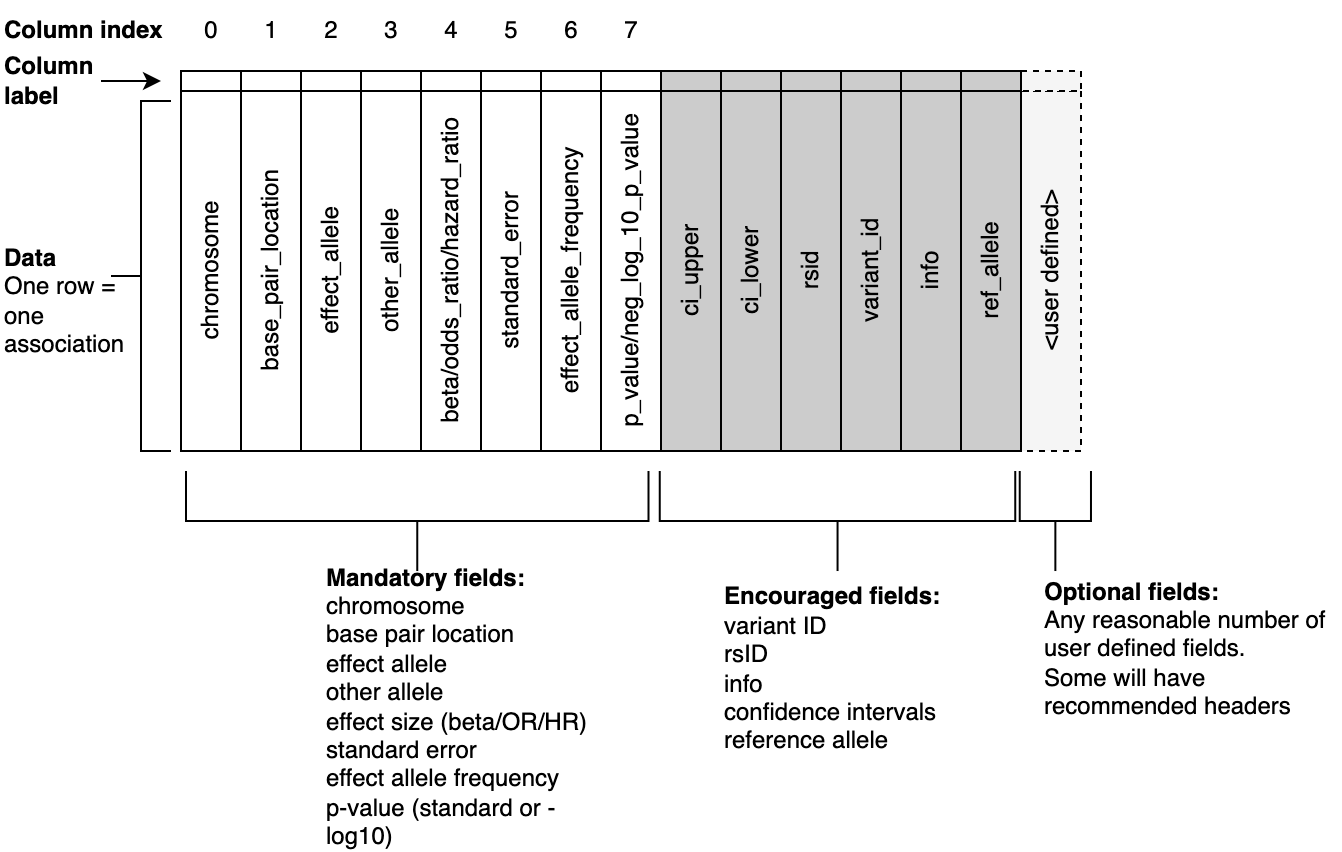
\includegraphics[width=\textwidth]{schematic}
 \label{fig:schematic}
\end{figure}
% ----------


% TABLE 1
\begin{landscape}
\begin{table}[h]
 \begin{threeparttable}
  \caption{Summary statistics field definitions}
  \centering
  \small
  \begin{tabularx}{\linewidth} { 
    | >{\hsize=0.7\hsize\centering\arraybackslash}X 
    | >{\hsize=1\hsize\centering\arraybackslash}X 
    | >{\hsize=1.9\hsize\centering\arraybackslash}X 
    | >{\hsize=0.4\hsize\centering\arraybackslash}X | } 
   \hline
   Field name & Description & Accepted values & Field type \\
   \hline
   chromosome & Column 0: Chromosome where the variant is located (X=23, Y=24, MT=25) & [1-25] & Mandatory\\
   base\_pair\_location & Column 1: The first position of the variant in the reference, counting on the bases, from 1 (1-based) & $x > 0$ & Mandatory\\
   effect\_allele & Column 2: Allele associated with the effect & [ACGT]+ & Mandatory\\
   other\_allele & Column 3: The non-effect allele & [ACGT]+ & Mandatory\\
   beta & Column 4: Effect size as beta & Numeric & Mandatory that either \textit{beta}, \textit{odds\_ratio} or \textit{hazard\_ratio} is given\\
   odds\_ratio & Column 4: Effect size as odds ratio & $x \ge 0$ & As above\\
   hazard\_ratio & Column 4: Effect size as hazard ratio & $x \ge 0$ & As above\\
   standard\_error & Column 5: Standard error & Numeric & Mandatory\\
   effect\_allele\_frequency & Column 6: Frequency of the effect allele & $0 \le x \le 1$\tnote{b} & Mandatory\\
   p\_value & Column 7: P-value of the association statistic & $0 \le x \le 1$ or $x \ge 0$ if p\_value is in the $-\log_{10}$ form\tnote{a} & Mandatory \\
   ci\_upper & Upper confidence interval & Numeric & Encouraged\\
   ci\_lower & Lower confidence interval & Numeric & Encouraged\\
   rsid & rsID & \^{}rs[0-9]+\$ & Encouraged\\
   variant\_id & An internal variant identifier formed by concatenating \textit{chromosome}, \textit{base\_pair\_location}, \textit{other\_allele} and \textit{effect\_allele} with underscores & [1-25]\_[0-9]+\_\texttt{(}[ACGT]+\_[ACGT]+\texttt{|}LONG\_STRING\texttt{)}\tnote{c} & Encouraged\\
   info & Imputation information metric & $0\le x\le 1$ & Encouraged\\
   n & Sample size & Numeric & Encouraged\\
   hm\_code & Harmonisation code, which can be looked up in the metadata to determine the transformation & Numeric & Only given in harmonised datasets\\
   \hline
  \end{tabularx}
   \begin{tablenotes}
    \item [a] If p-value is equal to 0, the precision of the p-value calculation must be given in the accompanying metadata.
    \item [b] Effect allele frequency can be rounded up to a threshold value defined in the metadata.
    \item [c] 'LONG\_STRING' can be used where allele string is too long to be represented. 
   \end{tablenotes}
   \label{tab:sum_stats_def}
  \end{threeparttable}
\end{table}
\end{landscape}
\normalsize
% -----------


\subsection{Summary statistics table contents}
Four fields in the summary statistics table, combined with the reference genome assembly provided in a metadata file (see below), unambiguously define the genetic variants (all field definitions can be found in Table 1). These fields are the chromosome (\textit{chromosome}), the genomic location position on the chromosome (\textit{base\_pair\_location}), the effect allele (\textit{effect\_allele}), and the non-effect allele (\textit{other\_allele}). Chromosome values are integers from 1 to 25, with chromosome X mapping to 23, chromosome Y to 24, and mitochondrial to 25. Genomic location is an integer value representing the first position of the variant in the reference genome, using 1-based indexing (see Figure~\ref{fig:variant_rep}) to maximise interoperability with variant call format (VCF) \cite{Danecek:2011ut}. The \textit{effect\_allele} field captures the allele for which the effect is associated with, while the \textit{other\_allele} field reports the non-effect allele. Both of the allele fields will contain allele strings, including cases where variants are insertions and deletions (see Figure~\ref{fig:variant_rep}). These four fields (\textit{chromosome, base\_pair\_location, effect\_allele, other\_allele}) are concatenated to populate the \textit{variant\_id} field and rsID can be stored in the \textit{rsid} field, but both fields are optional. 

All rows contain the following association statistics: p-value (\textit{p\_value}), the effect size (either \textit{beta}, \textit{odds\_ratio} or \textit{hazard\_ratio}), and the standard error (\textit{standard\_error}). Depending on the precision of software that performed the calculation of association, p-values in GWAS analyses may appear rounded to zero or one. This is particularly problematic where highly significant associations (e.g.\ $p < 10^{-300}$) are rounded to zero, preventing associations being ranked in order of significance. Calculation of accurate p-values is recommended where possible. Where this is not possible due to limitations of the software used, the GWAS-SSF requires the analysis and genotype imputation software and version to be present in the metadata, to help users of the summary statistics interpret these values. Alternatively, p-values can be expressed as negative log values, in which case the metadata field \textit{pvalueIsNegLog10} should be set to true. Effect allele frequency (\textit{effect\_allele\_frequency}) is a mandatory field. However, where privacy concerns might otherwise be a barrier to sharing the data, a cutoff may be specified in the metadata (\textit{effectAlleleFreqLowerLimit} field, see Table 2) so that frequencies below that cutoff are rounded-up to mask their true values. For example, \textit{effectAlleleFreqLowerLimit} = 0.01 in the metadata file would communicate that the lowest possible value for the effect allele frequency in this file is 0.01, and anything below this threshold has been rounded up to 0.01.


% TABLE 2
\begin{table}[h]
 \caption{Metadata field definitions}
 \centering
 \begin{tabularx}{\textwidth} { 
   | >{\hsize=1.4\hsize\centering\arraybackslash}X 
   | >{\hsize=1\hsize\centering\arraybackslash}X 
   | >{\hsize=1\hsize\centering\arraybackslash}X 
   | >{\hsize=0.6\hsize\centering\arraybackslash}X | } 
  \hline
  Field & Description & Accepted value & Mandatory \\
  \hline
  genomeAssembly & Genome assembly & GRCh/NCBI/UCSC value & Yes\\
  traitDescription & Author reported trait description & Text string (multiple possible) & Yes\\
  sampleSize & Sample size & Integer & Yes\\
  caseCount & Number of cases for case/control study & Integer & No, unless caseControlStudy is true\\
  controlCount & Number of controls for case/control study & Integer & No, unless caseControlStudy is true\\
  caseControlStudy & Flag whether the study is a case-control study & Boolean & No (default is false)\\
  sampleAncestry & Sample ancestry & Text string (multiple possible) & Yes\\
  genotypingTechnology & Genotyping technology & Text string (multiple possible) & Yes\\
  analysisSoftware & Software and version used for the association analysis & Text string & Yes if p-values of 0 given\\
  imputationPanel & Imputation panel & Text string & No\\
  imputationSoftware & Software used for imputation & Text string & No\\
  effectAlleleFreqLowerLimit & Lowest possible effect allele frequency & Numeric & No\\
  ancestryMethod & Method used to determine sample ancestry e.g. self-reported/genetically determined  & Text string (multiple possible) & No\\
  sortedByGenomicLocation & Flag whether the file is sorted by genomic location & Boolean & Yes\\
  effectStatistic & Indicate whether beta or odds ratio is used & beta/odds ratio/hazard ratio & Yes\\
  hmCodeDefinition & Description of harmonisation codes & Text string & Only given in harmonised datasets\\
  pvalueIsNegLog10 & Flag whether p value is given as $-\log_{10}$ & Boolean & No (default is false)\\
  adjustedCovariates & Any covariates the GWAS is adjusted for & Text string (multiple possible) & No\\
  ontologyMapping & Short form ontology terms describing the trait & Text string (multiple possible) & No\\
  \hline
 \end{tabularx}
 \label{tab:metadata_fields}
\end{table}
% ------------

\subsection{Summary statistics metadata}
An additional file accompanies the summary statistics data file containing metadata describing the summary statistics such as the name and md5sum of the summary statistics data file (see Section~\ref{metadata_example} for example) and the GWAS metadata itself, including sample and experimental metadata (Table 2),  thereby ensuring the reusability of the data. The metadata file fields can be expanded as needed in the future, and as with the summary statistics file, additional columns can be included as required. Sample metadata fields include descriptions of the trait under investigation and the sample size and ancestry. An additional field ancestryMethod can be used to indicate whether the ancestry descriptor is self-reported or genetically defined (encouraged). We recommend that ancestry is described according to the standardised framework guidelines described in Morales et al, 2018 \cite{PMID:29448949}. Every effort should be made to explicitly note whether the sample is admixed and the ancestral backgrounds that contribute to admixture. The trait description is free text and should include a clear description of the trait under study, including any relevant background characteristics of the study population, e.g.\ ``lung cancer in asthma patients''. Trait ontology terms can be stored in the metadata ontologyMapping field. The metadata file is in YAML format, which is ``a human-friendly data serialisation language for all programming languages'' (\url{https://yaml.org/}). There are both mandatory and encouraged metadata fields, which are detailed in Table~\ref{tab:metadata_fields}. 


\subsubsection{Metadata example} \label{metadata_example}

% METADATA EXAMPLE
\verbatiminput{./examples/0000123.yaml}
% ----------


% FIGURE 2
\begin{figure}[h]
 \centering
 \caption{Illustration of how variants are recorded in the summary statistics table for (a) SNP, (b) insertion, and (c) deletion alleles. Note that for insertions and deletions, the position of the base preceding the indel (the highlighted T at 8) is the position used to index the variant.}
 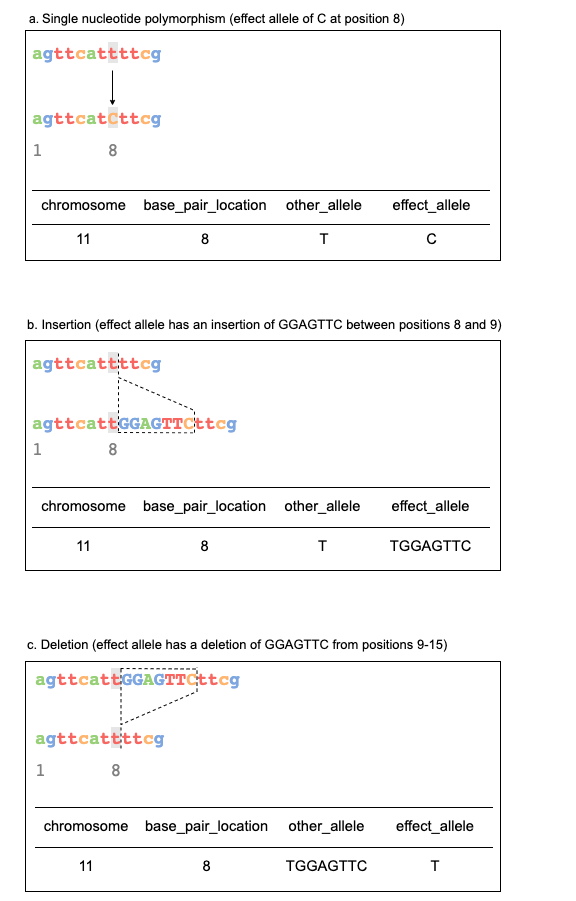
\includegraphics[width=0.8\textwidth]{variant_rep}
 \label{fig:variant_rep}
\end{figure}
% ----------

\bibliographystyle{abbrv}
\bibliography{refs}

% build notes: 
% pdflatex gwas-ssf_v0.1; bibtex gwas-ssf_v0.1; pdflatex gwas-ssf_v0.1; pdflatex gwas-ssf_v0.1

\end{document}
